\documentclass[tikz]{standalone}
\usepackage{tikz}
\usetikzlibrary{shapes}
\tikzstyle{mir}=[double]
\tikzstyle{d2}=[diamond,aspect=2,scale=0.5,draw]
\tikzstyle{d4}=[diamond,scale=0.5,rotate=45,draw]
\tikzstyle{d6}=[regular polygon, regular polygon sides=6,scale=0.5,draw]

\usetikzlibrary{calc}
\begin{document}
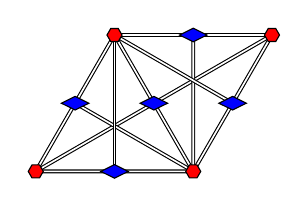
\begin{tikzpicture}
\coordinate (o) at (0, 0);
\coordinate (a) at (2, 0);
\coordinate (b) at (1, 1.732);
\coordinate (c) at (3, 1.732);

\draw (o)--(a)--(c)--(b)--(o) [mir];
\draw (a)--(b) [mir];
\draw (o)--(c) [mir];
\draw (a)--($(o)!.5!(b)$) [mir];
\draw (b)--($(o)!.5!(a)$) [mir];
\draw (a)--($(b)!.5!(c)$) [mir];
\draw (b)--($(c)!.5!(a)$) [mir];

\draw ($(o)!.5!(a)$) node [d2, fill=blue] {};
\draw ($(a)!.5!(b)$) node [d2, fill=blue] {};
\draw ($(b)!.5!(o)$) node [d2, fill=blue] {};
\draw ($(b)!.5!(c)$) node [d2, fill=blue] {};
\draw ($(c)!.5!(a)$) node [d2, fill=blue] {};

\draw (a) node [d6, fill=red] {};
\draw (b) node [d6, fill=red] {};
\draw (c) node [d6, fill=red] {};
\draw (o) node [d6, fill=red] {};

\end{tikzpicture}
\end{document}

